\documentclass[11pt,twocolumn]{article} 
\usepackage{geometry}
 \geometry{
  a4paper,
  left=17.5mm,
  right=17.5mm,
  bottom=15mm,
  top=15mm
 }
\usepackage[english]{babel}
\usepackage{tikz}
\usetikzlibrary{decorations.pathreplacing}

\title{\bf \Huge A Practical application of EOS projection geometry}
\author{{\bf \Large Anthony J. Lombard$^{1,2}$}\\
  $^1$ Medical Computing Team, Kitware Inc.,\\
  Albany, NY, USA\\
  $^2$ Department of Computer Science, Clarkson University,\\ 
  Potsdam, NY, USA
  }
\date{April 29th 2024}

\begin{document}
\maketitle

The report should contain an abstract within 300 words. The report should have a self-contained, citation-free abstract and state briefly the purpose of the research, methodology, key results and major conclusions. Abstract should be in a single paragraph with running sentences. Do not use any subheading or point list within the abstract. Also, non-standard or uncommon abbreviations should be avoided, but if essential they must be defined at their first mention in the abstract itself.  
\noindent
{\bf Keywords:} Authors are advised to write 3-5 keywords related to the project, separated by comma. 

\tikzset{XOR/.style={draw,circle,append after command={
        [shorten >=\pgflinewidth, shorten <=\pgflinewidth,]
        (\tikzlastnode.north) edge (\tikzlastnode.south)
        (\tikzlastnode.east) edge (\tikzlastnode.west)
        }
    }
}

\begin{tikzpicture}
  % Frontal emitter
  \draw (0,0) -- (5,.8);
  \draw (0,0) -- (5,-.8);
  \draw (5,.8) -- (5,-.8);
  \filldraw (0,0) circle (2pt) node[above,scale=0.8] at (0,0.1) {Frontal emitter};

  % Lateral emitter
  \draw (4,-4) -- (3.2,1);
  \draw (4,-4) -- (4.8,1);
  \draw (3.2,1) -- (4.8,1);
  \filldraw (4,-4) circle (2pt) node[below, scale=0.8] {Lateral emitter};

  % Isocenter
  \draw (4,0) node[XOR]{} node[above,scale=0.8] at (4, 0.15) {Isocenter};
\end{tikzpicture}

\begin{tikzpicture}
  \path[draw,decorate,decoration={brace}] (0,.8) -- (4,.8) node[midway,above]{Source to Isocenter Distance (SID)};
  % Frontal emitter
  \draw (0,0) -- (5,.8);
  \draw (0,0) -- (5,-.8);
  \draw (5,.8) -- (5,-.8);
  \filldraw (0,0) circle (2pt) node[above,scale=0.8] at (0,0.1) {};

  % Isocenter
  \draw (4,0) node[XOR]{} node[above,scale=0.8] at (4, 0.15) {};

  \path[draw,decorate,decoration={brace,mirror}] (0,-1) -- (5,-1) node[midway,below]{Source to Detector Distance (SDD)};
\end{tikzpicture}

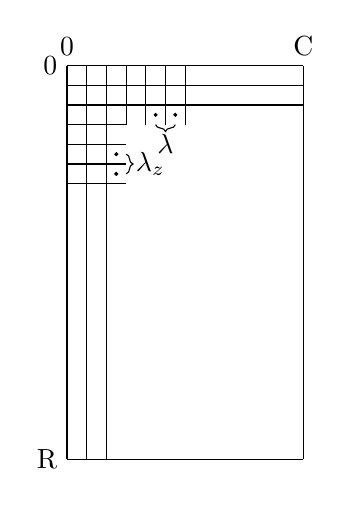
\begin{tikzpicture}
  \draw (0,0) node[above]{0} -- (3,0) node[above]{C};
  \draw (0,0) node[left] {0} -- (0,-5) node[left] {R};
  \draw (0,-5) -- (3,-5);
  \draw (3,-5) -- (3,0);

  % Horizontal Lines
  \draw (0,-0.25) -- (3,-.25);
  \draw (0,-0.5) -- (3,-.5);
  \draw (0,-0.75) -- (.75,-.75);
  \draw (0,-1) -- (.75,-1);
  \filldraw (0.625,-1.125) circle (0.5pt);
  \draw (0,-1.25) -- (.75,-1.25);
  \filldraw (0.625,-1.375) circle (0.5pt);
  \draw (0,-1.5) -- (.75,-1.5);

  \path[draw,decorate,decoration={brace}] (0.75 ,-1.125) -- (0.75,-1.375) node[midway,right]{$\lambda_z$};

  % Vertical Lines
  \draw (.25,0) -- (.25,-5);
  \draw (.5,0) -- (.5,-5);
  \draw (.75,0) -- (.75,-.75);
  \draw (1,0) -- (1,-.75);
  \filldraw (1.125,-.625) circle (0.5pt);
  \draw (1.25,0) -- (1.25,-.75);
  \filldraw (1.375,-.625) circle (0.5pt);
  \draw (1.5,0) -- (1.5,-.75);

  \path[draw,decorate,decoration={brace,mirror}] (1.125 ,-0.75) -- (1.375,-0.75) node[midway,below]{$\lambda$};
\end{tikzpicture}

\begin{equation}
  z = z_0 - \lambda_z * v
\end{equation}

\begin{equation}
  e_f = \{-sid,0,z\}
\end{equation}

\begin{equation}
  d_f = \{sdd-sid, \frac{(u - \frac{C}{2}) \cdot \lambda \cdot sdd}{sid},z\}
\end{equation}

\begin{equation}
  e_l = \{0,-sid,z\}
\end{equation}

\begin{equation}
  d_l = \{\frac{(u - \frac{C}{2}) \cdot \lambda \cdot sdd}{sid}, sdd-sid, z\}
\end{equation}

\section{Introduction}

We use the following equation
\begin{equation}
E = mc^2, \label{eqn:equation1}
\end{equation}
to estimate the energy produced during a nuclear reaction. 

The equation (\ref{eqn:equation1}) was derived by 


\section{Literature review}
This part should contain sufficient detail to reproduce reported data. It can be divided into subsections if several methods are described. Methods already published should be indicated by a reference [4], only relevant modifications should be described. Methodology should be written concisely in detail by maintaining continuity of the texts. 

\section{Theory and Calculation / Experimental set-up}

A theory section should extend, not repeat, the background to the article already dealt with in the Introduction and lay the foundation for further work. In contrast, a Calculation section represents a practical development from a theoretical basis. Do not add extensive basic definitions or well-known theories, instead highlight theoretical background and its specific usages in view of your work only.
\subsection{Mathematical Expressions and Symbols}
Mathematical expressions and symbols should be inserted using equation tool of Microsoft word. References may be added for used equations to support its authenticity, e.g. this result has been analysed using Fourier series [5].
\begin{equation}
f(x) = a_0 + \sum_{n=1}^\infty \left( a_n \cos {n\pi x\over L} + b_n \sin {n\pi x \over L} \right).
\end{equation}

\section{Results and Discussion}
This section may each be divided by subheadings or may be combined.  A combined Results and Discussion section is often appropriate.  This should explore the significance of the results of the work, don’t repeat them. Avoid extensive citations and discussion of published literature, instead discuss only recent literature for comparing your work to highlight novelty of the work in view of recent development and challenges in the field.

\subsection{Preparation of Figures and Tables}
You are supposed to embed all figures and tables at appropriate place within text. Figures and Tables should be numbered properly with descriptive title. Each Figure/Table must be explained within the text by referring to corresponding figure/table number. Max. 10 illustrations recommended, i.e., figures, graphs, tables are allowed in this report. All additional illustrations can be added to the Appendix/Supplemental Material.

\subsection{Formatting Tables}
Table should be prepared using table tool within the Microsoft word and cited consecutively in the text. Every table must have a descriptive title and if numerical measurements are given, the units should be included in the column heading. Formatting requirement has been summarized in the Table 1.


\begin{table}
\caption{Summary of formatting requirement for submitting paper in this journal.}

\begin{tabular}{|c|c|c|c|c|} \hline
Layout	& Size&	Margin  &	Footer &	 \\ 
 	&  &	(normal) &	 &	 \\  \hline
Font &	Article 	&Headings	&Reference	&Text \\ 
 &	Title	& 	& list	& \\ \hline
& & & & \\				\hline
Line  &	1.15	&1.15&	1.15	&1.15 \\ \hline
 Spacing &		&  &		&  \\ \hline
\end{tabular}
\end{table}


\subsection{Formatting Figures}
All figures should be cited in the paper in a consecutive order. Figures should be used in bitmap formats (TIFF, GIF, JPEG, etc.) with 300 dpi resolution at least unless the resolution is intentionally set to a lower level for scientific reasons. Figure 1 shows the logo of UCL.

 

\section{Conclusions}

Each report should contain a conclusion section within 250-450 words which may contain the major outcome of the work, highlighting its importance, limitation, relevance, application and recommendation. Conclusion should be written in continuous manner with running sentences which normally includes main outcome of the work, its application, limitation and recommendation. Do not use any subheading, citation, references to other part of the manuscript, or point list within the conclusion.

\section{Declarations}
\subsection{Acknowledgements}
All acknowledgments (if any) should be included here and may include list of peoples who contributed to the work in the manuscript but not listed in the author list. 
\cite{groisser2019geometry}


\bibliographystyle{plain}
\bibliography{manuscript_references}

\end{document}
